\documentclass[12pt]{article}
\usepackage[utf8]{inputenc}
\usepackage{amsmath}
\usepackage[slovene]{babel}
\usepackage{hyperref}
\title{Naloga 1}
\author{Gregor Kikelj}

\usepackage{natbib}
\usepackage{graphicx}
\usepackage{listings}

\begin{document}
\section{Naloga 1}
Iz vaj se spomnimo da je $T_n(x)-T_{n-1}(y)$ nerazcepen natanko tedaj ko je 
$D(n, n-1)=1$, kar pa je očitno vedno res, recimo po evklidovem algoritmu. Imamo torej $n \choose 2$
singularnih točk, ki pa so navadne dvojne točke, torej imajo po dve različni tangenti. 
Plot za $n=6$ in $n=10$ ker lahko :)

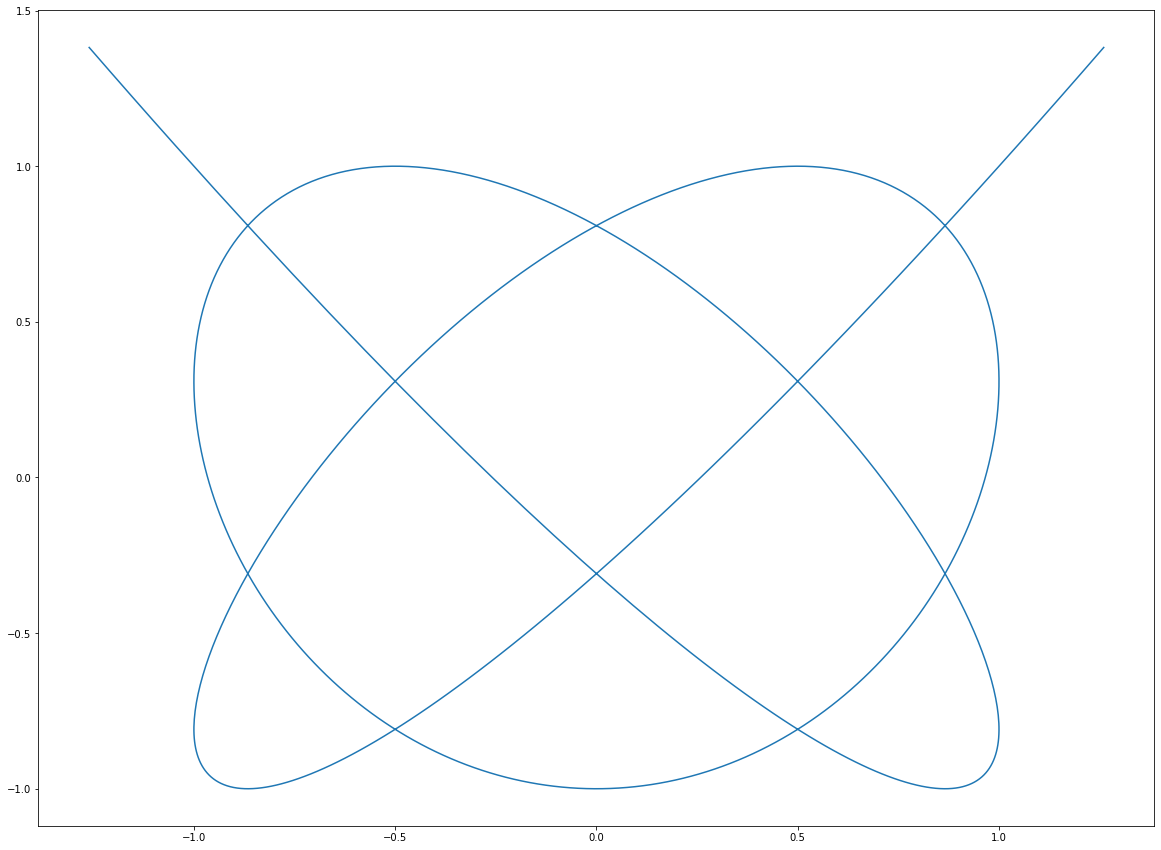
\includegraphics[scale=0.25]{plot6.png}

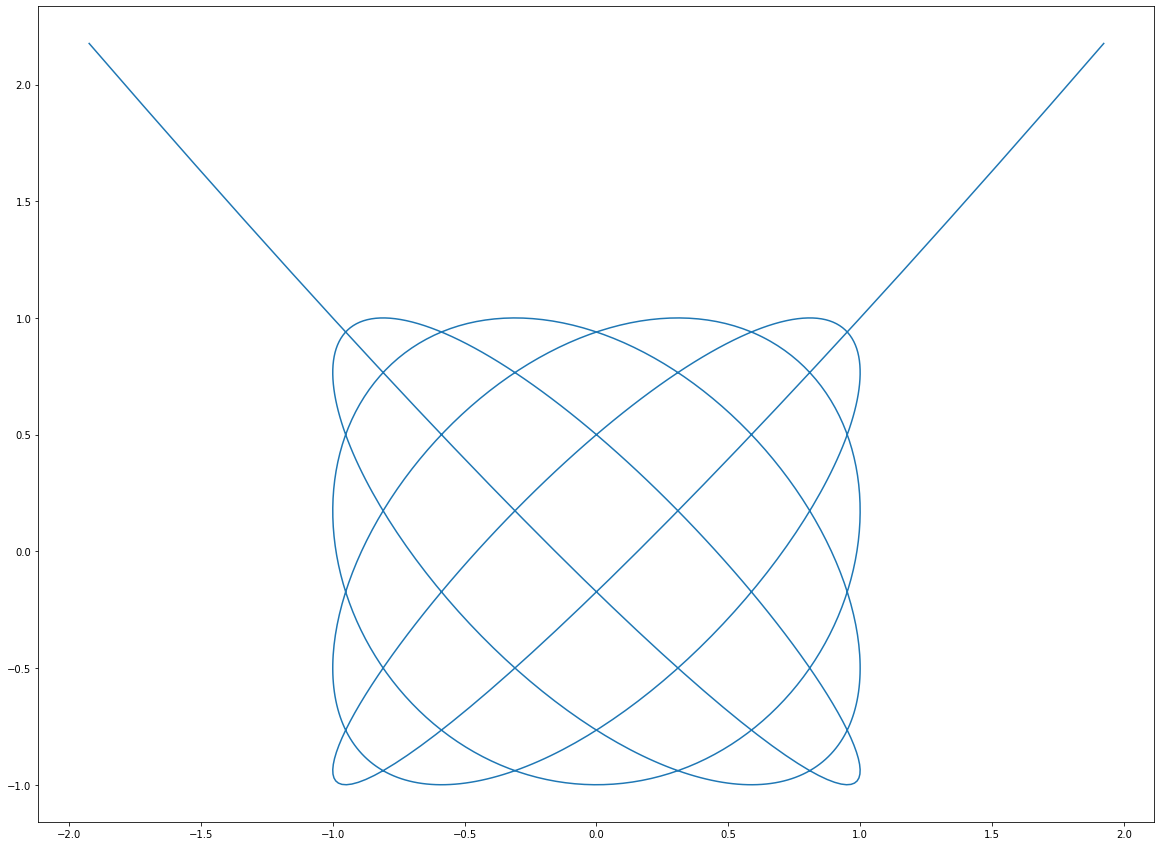
\includegraphics[scale=0.25]{plot10.png}
\end{document}
